% Mục 5.1: Bài toán phân tích phương sai ANOVA.
% Số liệu lấy từ generated/anova_*.tex, sinh bởi scripts/reports/report_anova.py.
% Dùng nguyên bộ dữ liệu cuối của Mục 3; mục này không sửa hay tạo thêm dữ liệu.
% Cần: booktabs, graphicx, listings, amsmath; macro \Anova... từ anova_numbers.tex.
% Khi ghép vào báo cáo chính: \setcounter{secnumdepth}{4} và
% \renewcommand{\theparagraph}{\thesubsubsection.\alph{paragraph}} để đánh số 5.1.2.a;
% thêm hai tài liệu lumley2002 và delacre2019 (xem preview_section5_anova.tex).

\subsection{Bài toán phân tích phương sai ANOVA}
\label{sec:anova}

\subsubsection{Đề xuất phương pháp}
\label{sec:anova-method}

Loại bộ nhớ đi theo thế hệ và phân khúc của card: DDR2 có ở các card ra đời 2003--2010,
khoảng \AnovaDdrThreeLaptopPercent\% card DDR3 là card laptop, còn GDDR5X chỉ có ở card cao
cấp ra đời 2016--2017. Vì vậy có thể dùng loại bộ nhớ để chia nhóm khi so sánh công suất.

\begin{center}
\fbox{\parbox{0.92\linewidth}{\textbf{Bài toán.} Với mức ý nghĩa $\alpha = 0{,}05$, công
suất tối đa trung bình (\texttt{max\_power\_w}) có khác nhau giữa các nhóm loại bộ nhớ
(\texttt{memory\_type\_group}) hay không?}}
\end{center}

Bài toán dùng nguyên bộ dữ liệu cuối của Mục~3, gồm \AnovaRows{} card thuộc \AnovaGroups{}
nhóm DDR2, DDR3, GDDR3, GDDR5 và GDDR5X. Nhóm ``Other'' (\AnovaOtherRows{} card) không được
đưa vào so sánh: nhóm này gộp các loại bộ nhớ không liên quan đến nhau (DDR, GDDR2, GDDR4,
HBM), nên trung bình của nó không đại diện cho loại bộ nhớ nào. Theo Bảng~\ref{tab:anova-groups}
và Hình~\ref{fig:anova-box}, công suất trung bình tăng dần từ DDR2 đến GDDR5X, còn độ phân tán
và cỡ nhóm chênh nhau nhiều. Nhóm GDDR5X có \AnovaGddrFiveXCards{} card, chủ yếu là các phiên
bản GTX~1080 và GTX~1080~Ti do nhiều hãng lắp ráp.

\begin{table}[htbp]
  \centering
  \caption{Công suất tối đa (W) theo nhóm loại bộ nhớ; $p$ là kết quả kiểm định
    Shapiro--Wilk ở Mục~\ref{par:anova-normal}}
  \label{tab:anova-groups}
  \begin{tabular}{l r r r r r}
    \toprule
    \textbf{Nhóm} & \textbf{Số card} & \textbf{Trung bình} & \textbf{Độ lệch chuẩn}
      & \textbf{Trung vị} & \textbf{\boldmath$p$} \\
    \midrule
    \csname @@input\endcsname generated/anova_groups.tex
    \bottomrule
  \end{tabular}
\end{table}

\begin{figure}[htbp]
  \centering
  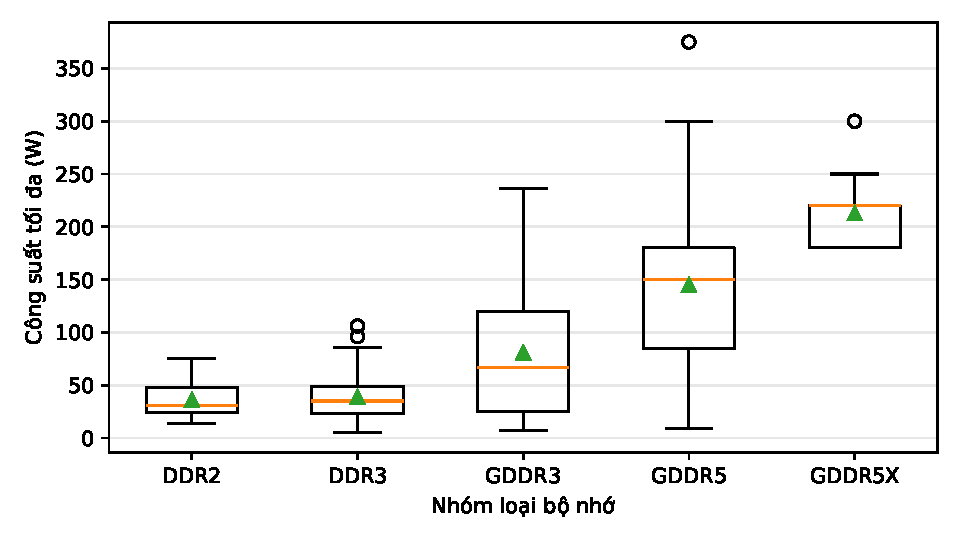
\includegraphics[width=0.75\linewidth]{generated/anova_boxplot.pdf}
  \caption{Công suất tối đa theo nhóm loại bộ nhớ. Vạch cam là trung vị, tam giác là trung
    bình, chấm tròn là giá trị cách tứ phân vị gần nhất quá 1,5 lần khoảng tứ phân vị.}
  \label{fig:anova-box}
\end{figure}

Ta so sánh trung bình của năm nhóm bằng phân tích phương sai (ANOVA) một nhân tố. Gọi
$\mu_1, \dots, \mu_5$ lần lượt là công suất trung bình của các nhóm DDR2, DDR3, GDDR3, GDDR5
và GDDR5X. Cặp giả thuyết là
\[
  H_0: \mu_1 = \mu_2 = \dots = \mu_5, \qquad
  H_1: \text{tồn tại } i \ne j \text{ sao cho } \mu_i \ne \mu_j.
\]

ANOVA một nhân tố cần ba điều kiện: công suất trong mỗi nhóm có phân phối chuẩn, các nhóm có
phương sai bằng nhau, và các quan sát độc lập. Hai điều kiện đầu được kiểm tra ở
Mục~\ref{par:anova-normal} và~\ref{par:anova-levene}. Điều kiện thứ ba không thỏa: nhiều card
là phiên bản của cùng một chip do các hãng khác nhau lắp ráp và thường được ghi cùng một công
suất. Cột \texttt{architecture} chỉ có \AnovaArchLabels{} giá trị khác nhau cho \AnovaRows{}
card; riêng nhóm GDDR5X chỉ có \AnovaGddrFiveXArchLabels. Do đó các giá trị $p$ ở mục này gần
như chắc chắn nhỏ hơn giá trị đúng, các khoảng tin cậy hẹp hơn, và kết quả kiểm định cần được
diễn giải thận trọng. Khác biệt giữa các nhóm trước hết là khác biệt mô tả trong mẫu quan sát.
Đây là hạn chế chính của bài toán.

Hạn chế thứ hai đến từ việc loại dòng khuyết ở Mục~3. Nhóm GDDR3 chỉ còn \AnovaGddrThreeKept{}
trong \AnovaGddrThreeWithPower{} card có ghi công suất, và trung bình của nhóm là
\AnovaGddrThreeMeanKept~W, so với \AnovaGddrThreeMeanAll~W khi tính trên mọi card có ghi công
suất. Các nhóm còn lại gần như không đổi, nên thứ tự giữa các nhóm vẫn giữ nguyên.

\subsubsection{Phân tích ANOVA}

\paragraph{Kiểm tra điều kiện phân phối chuẩn.}
\label{par:anova-normal}
Đặt $H_0$: công suất trong nhóm có phân phối chuẩn; $H_1$: không có phân phối chuẩn.
Shapiro--Wilk bác bỏ $H_0$ ở cả năm nhóm (Bảng~\ref{tab:anova-groups}), nên điều kiện chuẩn
không thỏa. Sai lệch này có thật, không chỉ do kiểm định nhạy khi mẫu lớn: trên đồ thị Q--Q
(Hình~\ref{fig:anova-qq}), các điểm ở hai đầu lệch khỏi đường thẳng, và
\AnovaGddrFiveXLevelCards{} trong \AnovaGddrFiveXCards{} card GDDR5X có công suất đúng bằng một
trong ba mức \AnovaGddrFiveXLevels~W.

Dù vậy vẫn có thể dùng ANOVA, vì thống kê $F$ khá bền với vi phạm giả định chuẩn khi các nhóm
đủ lớn: theo định lý giới hạn trung tâm, trung bình mẫu của mỗi nhóm có phân phối xấp xỉ chuẩn
\cite{lumley2002}. Nhóm nhỏ nhất (\AnovaSizeMinGroup) có \AnovaSizeMin{} card. Với GDDR5X, lập
luận này yếu hơn vì nhóm chỉ gồm vài sản phẩm.

\begin{figure}[htbp]
  \centering
  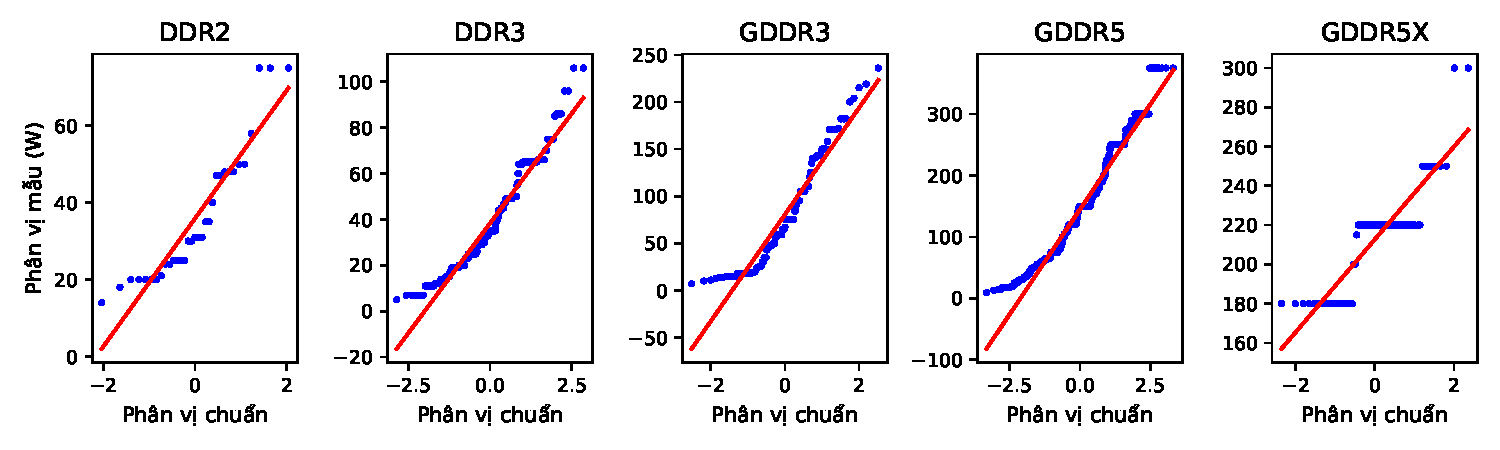
\includegraphics[width=\linewidth]{generated/anova_qq.pdf}
  \caption{Đồ thị Q--Q chuẩn của công suất trong từng nhóm; đường đỏ là đường tham chiếu của
    phân phối chuẩn.}
  \label{fig:anova-qq}
\end{figure}

\paragraph{Kiểm định tính đồng nhất về phương sai.}
\label{par:anova-levene}
Đặt $H_0$: $\sigma_1^2 = \dots = \sigma_5^2$; $H_1$: có ít nhất một phương sai khác. Kiểm
định Levene dùng trung vị (Brown--Forsythe) cho $F_{\mathrm{BF}} = \AnovaLeveneW$ với bậc tự do
$(\AnovaDfBetween;\ \AnovaDfWithin)$, $p < 0{,}001$, nên ta bác bỏ $H_0$. Độ lệch chuẩn của
\AnovaSdMaxGroup{} gấp \AnovaSdRatio{} lần của \AnovaSdMinGroup.

ANOVA cổ điển vẫn là phân tích chính. Nhóm lớn nhất (GDDR5) cũng là nhóm có phương sai lớn
nhất, nên $\mathrm{MSW}$ bị kéo lên và $F$ cổ điển có xu hướng khó bác bỏ $H_0$ hơn.
Mục~\ref{par:anova-check} kiểm tra lại bằng Welch ANOVA và Games--Howell, hai phương pháp không
cần phương sai bằng nhau.

\paragraph{Kiểm định ANOVA.}
\label{par:anova-test}
Từ Bảng~\ref{tab:anova-classic}, thống kê kiểm định và miền bác bỏ là
\[
  F = \frac{\mathrm{MSB}}{\mathrm{MSW}} = \AnovaClassicF, \qquad
  W_\alpha = \bigl(F_{0{,}95;\,\AnovaDfBetween;\,\AnovaDfWithin};\ +\infty\bigr)
    = (\AnovaClassicFCritical;\ +\infty).
\]
Với giả định các quan sát độc lập và phương sai bằng nhau, $F$ thuộc miền bác bỏ và
$p < 0{,}001$, nên ta bác bỏ $H_0$: có ít nhất hai nhóm loại bộ nhớ có công suất trung bình khác
nhau. Hai giả định này không thỏa (Mục~\ref{sec:anova-method} và~\ref{par:anova-levene}), nên
kết luận chịu hạn chế đã nêu.

\begin{table}[htbp]
  \centering
  \caption{Bảng ANOVA một nhân tố cho công suất theo nhóm loại bộ nhớ}
  \label{tab:anova-classic}
  \small
  \begin{tabular}{l r r r r r}
    \toprule
    \textbf{Nguồn biến thiên} & \textbf{\shortstack{Tổng\\bình phương}}
      & \textbf{\shortstack{Bậc\\tự do}} & \textbf{\shortstack{Trung bình\\bình phương}}
      & $F$ & $p$ \\
    \midrule
    Giữa các nhóm & $\mathrm{SSB} = \AnovaSsBetween$ & \AnovaDfBetween
      & $\mathrm{MSB} = \AnovaMsBetween$ & \AnovaClassicF & $<$ 0,001 \\
    Trong các nhóm & $\mathrm{SSW} = \AnovaSsWithin$ & \AnovaDfWithin
      & $\mathrm{MSW} = \AnovaMsWithin$ & & \\
    Tổng & $\mathrm{SST} = \AnovaSsTotal$ & \the\numexpr\AnovaDfBetween+\AnovaDfWithin\relax
      & & & \\
    \bottomrule
  \end{tabular}
\end{table}

Tỉ số $\eta^2 = \mathrm{SSB}/\mathrm{SST} = \AnovaEtaSq$: khác biệt giữa các nhóm chiếm
khoảng \AnovaEtaSqPercent\% tổng biến thiên của công suất. Các lệnh Python dùng trong mục này
được tóm tắt ở Đoạn code~\ref{lst:anova}.

\begin{lstlisting}[language=Python, float=htbp, columns=fixed, label={lst:anova},
  caption={Các kiểm định chính của Mục~\ref{sec:anova} (rút gọn từ \texttt{report\_anova.py})}]
from scipy import stats
from statsmodels.stats.multicomp import pairwise_tukeyhsd
from statsmodels.stats.oneway import anova_oneway

gpu = gpu[gpu["memory_type_group"] != "Other"]
y, g = gpu["max_power_w"], gpu["memory_type_group"]
groups = [y[g == level] for level in g.unique()]
[stats.shapiro(v) for v in groups]      # normality in each group
stats.levene(*groups, center="median")  # equal variances (Brown-Forsythe)
stats.f_oneway(*groups)                 # one-way ANOVA
pairwise_tukeyhsd(y, g.astype(str))     # Tukey HSD
anova_oneway(y, g, use_var="unequal")   # check: Welch ANOVA
stats.kruskal(*groups)                  # check: Kruskal-Wallis
\end{lstlisting}

\paragraph{Kiểm tra sự khác biệt giữa các nhóm.}
\label{par:anova-posthoc}
\begin{table}[!htbp]
  \centering
  \caption{So sánh từng cặp bằng Tukey HSD (chênh lệch = nhóm trước trừ nhóm sau, W)}
  \label{tab:anova-tukey}
  \begin{tabular}{l r c r l}
    \toprule
    \textbf{Cặp} & \textbf{Chênh lệch} & \textbf{KTC 95\%} & \textbf{\boldmath$p$ hiệu chỉnh}
      & \textbf{Kết luận $H_0$} \\
    \midrule
    \csname @@input\endcsname generated/anova_tukey.tex
    \bottomrule
  \end{tabular}
\end{table}
Vì $H_0$ đã bị bác bỏ, ta so sánh $\binom{5}{2} = \AnovaPairs$ cặp nhóm bằng Tukey HSD, có
hiệu chỉnh giá trị $p$ cho việc so sánh nhiều lần. Cỡ nhóm khác nhau nên ta dùng phiên bản
Tukey--Kramer. Với mỗi cặp, $H_0$: $\mu_i = \mu_j$; $H_1$: $\mu_i \ne \mu_j$. Tukey cũng giả định
phương sai bằng nhau, nên với lý do như ở Mục~\ref{par:anova-levene}, phương pháp này khó bác
bỏ $H_0$ hơn ở các cặp gồm những nhóm có phương sai nhỏ.

Theo Bảng~\ref{tab:anova-tukey}, \AnovaPairsSignificant{} trong \AnovaPairs{} cặp có trung
bình khác nhau có ý nghĩa thống kê. Riêng cặp \AnovaPairsNotSignificant{} có khoảng tin cậy
$[\AnovaDdrThreeMinusDdrTwoLow;\ \AnovaDdrThreeMinusDdrTwoHigh]$~W chứa 0, nên chưa đủ bằng
chứng để nói hai nhóm này khác nhau. Khoảng này rộng chủ yếu vì $\mathrm{MSW}$ chung bị phương
sai lớn của GDDR5 kéo lên. Games--Howell dùng phương sai riêng của từng nhóm và cho khoảng hẹp
hơn, $[\AnovaDdrThreeMinusDdrTwoGamesLow;\ \AnovaDdrThreeMinusDdrTwoGamesHigh]$~W, nhưng khoảng
này cũng coi các card là độc lập. Xếp theo công suất trung bình tính trên từng card (dấu
$\approx$ nghĩa là không phát hiện khác biệt):
\[
  \text{DDR2} \approx \text{DDR3} < \text{GDDR3} < \text{GDDR5} < \text{GDDR5X}.
\]

\paragraph{Kiểm tra lại kết luận.}
\label{par:anova-check}
Welch ANOVA không cần phương sai bằng nhau và kiểm soát sai lầm loại I gần mức $\alpha$ khi
phương sai và cỡ nhóm không đều \cite{delacre2019}. Phương pháp này cho $F = \AnovaWelchF$ với
bậc tự do $(\AnovaWelchDfOne;\ \AnovaWelchDfTwo)$, thuộc miền bác bỏ
$(\AnovaWelchFCritical;\ +\infty)$, nên vẫn bác bỏ $H_0$. Games--Howell cũng cho
\AnovaGamesSignificant{} trong \AnovaPairs{} cặp khác nhau, và cặp không khác nhau vẫn là
\AnovaGamesNotSignificant. Kruskal--Wallis, không cần giả định chuẩn, bác bỏ giả thuyết các
nhóm có cùng phân phối ($H = \AnovaKruskalH$, $p < 0{,}001$). Cả ba phương pháp vẫn giả định
các quan sát độc lập, nên không khắc phục được hạn chế ở Mục~\ref{sec:anova-method}.

\subsubsection{Kết luận}

Trong mẫu quan sát, công suất tối đa trung bình khác nhau rõ giữa các nhóm loại bộ nhớ. ANOVA
ở mức ý nghĩa 0,05 bác bỏ giả thuyết các nhóm có cùng trung bình, Welch ANOVA cho cùng kết
luận, và Kruskal--Wallis cho thấy phân phối công suất cũng khác nhau. Vì các quan sát không độc
lập và phương sai không bằng nhau, các kết quả kiểm định này cần được diễn giải thận trọng.
Tính trên từng card, card GDDR5X có công suất trung bình cao hơn card GDDR5 khoảng
\AnovaGddrFiveXMinusGddrFive~W (KTC 95\%:
$[\AnovaGddrFiveXMinusGddrFiveLow;\allowbreak\ \AnovaGddrFiveXMinusGddrFiveHigh]$~W). Khoảng này
coi các card là độc lập nên hẹp hơn thực tế, và con số chủ yếu phản ánh hai dòng GTX~1080 và
GTX~1080~Ti. Giữa DDR2 và DDR3 chưa phát hiện khác biệt.

Kết quả chỉ cho thấy loại bộ nhớ có liên hệ với công suất. Card dùng bộ nhớ đời mới thường
cũng dùng chip mạnh hơn, và card laptop tập trung nhiều ở nhóm DDR3, nên không thể quy hết khác
biệt giữa các nhóm cho loại bộ nhớ; ANOVA một nhân tố chỉ xét một yếu tố nên không tách được
các ảnh hưởng này. Kết luận chỉ áp dụng cho card đồ họa rời (desktop và laptop) trong bộ dữ liệu, chủ yếu
ra đời 2006--2017, và không bao gồm nhóm ``Other''.
